\documentclass[11pt,a4paper]{article}

\usepackage[margin=1.1in]{geometry}
\usepackage{amsmath,amssymb,amsthm}
\usepackage{mathtools}
\usepackage{xcolor}
\usepackage{hyperref}
\usepackage{booktabs}
\usepackage{array}
\usepackage{tabularx}
\usepackage{enumitem}
\usepackage{graphicx}
\usepackage{float}
\usepackage{caption}
\usepackage{tcolorbox}
\usepackage{fancyhdr}
\usepackage{titlesec}
\usepackage{setspace}
\usepackage{parskip}
\usepackage{tikz}
\usepackage{pgfplots}
\pgfplotsset{compat=1.18}
\usetikzlibrary{arrows.meta,positioning,shapes.geometric,fit,backgrounds,calc}

\hypersetup{
  colorlinks=true,
  linkcolor=blue!70!black,
  citecolor=blue!70!black,
  urlcolor=blue!70!black,
}

% Theorem environments
\theoremstyle{plain}
\newtheorem{theorem}{Theorem}[section]
\newtheorem{lemma}[theorem]{Lemma}
\newtheorem{corollary}[theorem]{Corollary}
\newtheorem{proposition}[theorem]{Proposition}

\theoremstyle{definition}
\newtheorem{definition}[theorem]{Definition}
\newtheorem{axiom}[theorem]{Axiom}
\newtheorem{example}[theorem]{Example}

\theoremstyle{remark}
\newtheorem{remark}[theorem]{Remark}

% Custom math operators
\DeclareMathOperator{\Sign}{Sign}
\DeclareMathOperator{\Grammar}{Grammar}
\DeclareMathOperator{\Motif}{Motif}
\DeclareMathOperator{\Endo}{\mathcal{E}}
\DeclareMathOperator{\interior}{int}
\DeclareMathOperator{\dom}{dom}
\newcommand{\R}{\mathbb{R}}
\newcommand{\N}{\mathbb{N}}
\newcommand{\B}{\{0,1\}}
\newcommand{\Traj}{\mathbf{Traj}}
\newcommand{\Ep}{\mathbf{Ep}}
\newcommand{\Obs}{\mathcal{O}}
\newcommand{\He}{\mathcal{H}}
\newcommand{\Ga}{\mathcal{G}}
\newcommand{\Mo}{\mathcal{M}}
\newcommand{\Ph}{\Phi}
\newcommand{\norm}[1]{\left\|#1\right\|}
\newcommand{\abs}[1]{\left|#1\right|}

% Header/footer
\pagestyle{fancy}
\fancyhf{}
\fancyhead[L]{\small\textit{DSFB Structural Semiotics Calculus: Endoduction as a Fourth Mode of Inference}}
\fancyhead[R]{\small\textit{Invariant Forge LLC}}
\fancyfoot[C]{\thepage}
\renewcommand{\headrulewidth}{0.4pt}

% Section formatting
\titleformat{\section}{\large\bfseries}{\thesection}{1em}{}
\titleformat{\subsection}{\normalsize\bfseries}{\thesubsection}{1em}{}
\titleformat{\subsubsection}{\normalsize\itshape}{\thesubsubsection}{1em}{}

% Notice box
\tcbuselibrary{breakable,skins}
\newtcolorbox{noticebox}{
  colback=gray!8,
  colframe=gray!50,
  boxrule=0.5pt,
  arc=2pt,
  breakable,
  left=6pt, right=6pt, top=4pt, bottom=4pt,
}

\begin{document}

% ============================================================
%  TITLE PAGE
% ============================================================

\begin{center}
{\LARGE\bfseries DSFB Structural Semiotics Calculus}\\[0.6em]
{\large Endoduction as a Fourth Mode of Inference:\\
Formal Syntax, Composition Rules, and Provable Properties\\
of Endoductive Inference over Residual Trajectories}\\[1.2em]
{\normalsize Riaan de Beer}\\
{\small\texttt{riaan@invariantforge.net}}\\
{\small Chief Research Advisor, Invariant Forge LLC}\\
{\small ORCID: 0009-0006-1155-027X}\\[0.8em]
{\small DOI: \texttt{10.5281/zenodo.XXXXXXX} \quad (pending deposit)}\\
{\small \url{https://github.com/infinityabundance/dsfb/tree/main/crates/dsfb-semiotics-calculus}}\\[0.5em]
{\small Version 1.0 \quad April 2026}
\end{center}

\vspace{0.5em}
\begin{noticebox}
\textbf{Prior Art Notice.} This work constitutes prior art under 35~U.S.C.~\S~102 and is
timestamped via public GitHub repository \url{https://github.com/infinityabundance/dsfb} and
Zenodo DOI (pending). All rights reserved to prior-art date of public deposit.
Export Control: This document contains no controlled technical data within the meaning of ITAR
(22~C.F.R.~\S\S~120--130) or EAR (15~C.F.R.~\S\S~730--774). Foreign National Notice: This paper is
published as open academic research. Prior art under 35~U.S.C.~\S~102 is established by the Zenodo
timestamp and GitHub commit hash. Governing law: Delaware, USA.
\end{noticebox}

% ============================================================
%  EXECUTIVE SUMMARY (Licensing Synopsis)
% ============================================================
\begin{tcolorbox}[colback=blue!4, colframe=blue!55, boxrule=0.8pt, arc=4pt,
  left=8pt, right=8pt, top=7pt, bottom=7pt,
  title={\textbf{Executive Summary — Licensing Synopsis}},
  fonttitle=\normalsize\bfseries, coltitle=blue!10!black]

\textbf{What this paper establishes.}
The DSFB Structural Semiotics Calculus (DSSC) is a typed algebraic framework that turns
residual streams already produced by any incumbent monitoring system into deterministic,
auditable, typed structural interpretations — without modifying, replacing, or accessing
the system that produces them.

\medskip
\textbf{The delta over existing diagnostic approaches.}
Abduction-based systems (FDC libraries, ML classifiers, neural networks) are dictionaries:
if the fault is not in the dictionary, the system is either mute or wrong. The DSSC is an
\textbf{alphabet}: even for an event it has never seen, it spells out the complete structural
characterization, proves why it is there, and guarantees the spelling process will not
affect the observed system. This is Bounded Completeness (Theorem~\ref{thm:completeness})
and No Silent Failure (Corollary~\ref{cor:no_silence}) — proven, not claimed.

\medskip
\textbf{Three deployment arguments, each theorem-backed.}

\smallskip
\noindent\textbf{1. No cold-start problem.}
Phase~I can be completed with an empty heuristics bank. On Day~1, the system operates as
a \emph{Deterministic Structural Logger}: it records the structural phonemes of system
behavior (sign evolution, grammar path, ADD invariants) before any fault names are known.
Every $(\mathtt{Unknown}, \tau_\phi)$ episode is a complete forensic record.
\hfill\textit{(Prop.~\ref{prop:empty_bank})}

\smallskip
\noindent\textbf{2. Forensic AI: every output is a mathematical proof.}
Every episode carries a provenance tag $\tau_\phi$ — a replayable derivation tree from
residual onset to diagnostic conclusion. Unlike neural network outputs, $\tau_\phi$ is
independently verifiable, self-contained, and maps directly to DO-178C \S6.3,
MIL-STD-882E Task~102, and IEC~61508-3 \S7.9 audit requirements.
\hfill\textit{(Thm.~\ref{thm:audit})}

\smallskip
\noindent\textbf{3. Observer-only overlay — zero integration risk.}
No controller access. No architecture review. No rollback procedure. The read-only
constraint is enforced structurally by functor purity — not by policy or code review.
Remove the DSSC at any time; the observed system is mathematically unchanged.
\hfill\textit{(Cor.~\ref{cor:noninterference})}

\medskip
\textbf{Safety-case properties, each theorem-backed.}\\[0.2em]
\begin{tabular}{@{}lll@{}}
Read-only, zero side effects & Functor purity & Thm.~\ref{thm:functor} \\
Replayable audit certificate & Provenance tag $\tau_\phi$ & Thm.~\ref{thm:audit} \\
No silent failure & Bounded completeness & Cor.~\ref{cor:no_silence} \\
Day-one value (empty library) & Structural logger & Prop.~\ref{prop:empty_bank} \\
Graceful noise degradation & Linear fragmentation & Lem.~\ref{lem:graceful_degradation} \\
Reversible integration & Observer functor & Cor.~\ref{cor:noninterference} \\
\end{tabular}

\medskip
\textbf{Licensing contact.}\ \texttt{licensing@invariantforge.net}\quad
Invariant Forge LLC (Delaware~No.~10529072)
\end{tcolorbox}

\bigskip

% ============================================================
%  ABSTRACT
% ============================================================
\section*{Abstract}

We introduce the \emph{DSFB Structural Semiotics Calculus} (DSSC), a typed algebraic framework
that unifies residual sign semantics, admissibility envelopes, grammar-state machines, motif
rewriting, and endoductive inference into a single coherent formal system. Building directly on
the algebraic primitives of Algebraic Deterministic Dynamics (ADD) and the Drift--Slew Fusion
Bootstrap (DSFB) estimation layer, the calculus supplies deterministic composition rules,
operational semantics in the style of structured operational semantics (SOS), and provable
meta-properties without stochastic assumptions. Endoduction is formalized as a fourth inference
mode, distinct from deduction, induction, and abduction, with explicit soundness and bounded
completeness guarantees under discrete-time, finite-dimensional, bounded-noise assumptions. The
framework yields replay-deterministic, non-interfering observers whose outputs are typed episodes
over abstract residual trajectories. We prove: (i) finite-time envelope exit under ADD dynamics
(generalized from prior work); (ii) monotonicity of the heuristics bank under augmentation; (iii)
bounded fragmentation under bounded noise; (iv) categorical non-interference via a functor
$\Obs : \Traj \to \Ep$; and (v) commutativity of ADD rewriting with grammar transitions. Every
prior DSFB and ADD paper is an instance of this single calculus. This paper serves as the
canonical foundational reference for all DSFB instantiations.

\textbf{Keywords:} deterministic inference, structural semiotics, residual calculus, endoduction,
typed operational semantics, non-interfering observer, admissibility envelope, algebraic
deterministic dynamics, grammar automata, motif rewriting.

% ============================================================
%  IP NOTICE
% ============================================================
\begin{noticebox}
\textbf{IP Notice.} The theoretical framework, formal constructions, and supervisory methods
described herein constitute proprietary Background IP of Invariant Forge LLC (Delaware LLC
No.~10529072), with prior art established by this publication and earlier Zenodo DOI publications
by the same author. Commercial deployment, integration, sublicensing, or derivative use of the
framework---including re-derivation by abstraction, equivalent reformulation, notation substitution,
or domain translation---requires a separate written license from Invariant Forge LLC.
Licensing inquiries: \texttt{licensing@invariantforge.net}
\end{noticebox}

\tableofcontents
\newpage

% ============================================================
%  SECTION 1: INTRODUCTION
% ============================================================
\section{Introduction}
\label{sec:intro}

\subsection{Motivation}

The DSFB research program now spans more than twenty published papers and Zenodo-deposited
prior-art filings covering aerospace navigation~\cite{dsfb_nav}, semiconductor process
control~\cite{dsfb_semi}, battery health monitoring~\cite{dsfb_battery}, causal dynamics~\cite{dscd},
algebraic structural modeling~\cite{add}, and more than a hundred additional application
domains~\cite{dsfb_survey}. Each paper instantiates a common pattern: take residual streams
already produced by an incumbent probabilistic estimator, and extract from them a typed,
deterministic, human-readable structural interpretation. Each paper cites the same handful of
core theorems---Law~1 (Structural Detectability), Theorem~1 (Finite-Time Envelope Exit),
Theorem~9 (Deterministic Interpretability)---and each extends or instantiates the heuristics
engine and grammar layer introduced in the foundational semiotics paper~\cite{dsfb_semiotics}.

What has been absent is a unified mathematical object in which all of these are instances. The
present paper supplies that object: the \emph{DSFB Structural Semiotics Calculus} (DSSC), a
typed algebraic calculus with a formal syntax, deterministic operational semantics, composition
operators, and a complete set of provable properties.

\subsection{Central Claim}

The central claim of this paper is modest and precise: every prior DSFB and ADD paper is a
specialization of the DSSC to a particular domain, residual type, or envelope family. No prior
result is invalidated; all prior theorems are subsumed as instances of theorems stated here in
full generality.

\subsection{Scope and Non-Claims}

The DSSC is a \emph{purely theoretical} contribution. It assumes:
\begin{enumerate}[nosep]
  \item Discrete-time residual trajectories over finite-dimensional normed spaces.
  \item Bounded noise: $\norm{w(k)} \leq w_{\max}$ for all $k$.
  \item A finite admissibility envelope family and a finite grammar alphabet.
  \item ADD growth invariants as defined in~\cite{add}.
\end{enumerate}
The calculus does not address continuous-time or infinite-dimensional systems, does not make
completeness claims for arbitrary dynamical systems, and does not constitute a claim of
superiority over any probabilistic inference method in any deployment setting. It is a
foundational mathematical framework.

\subsection{Contributions}

This paper makes five new contributions:
\begin{enumerate}[nosep]
  \item \textbf{Unified typed syntax.} A single formal language with types for all DSFB objects:
    residual signs, envelopes, grammar states, motifs, episodes, and provenance tags.
  \item \textbf{Operational semantics.} A complete small-step SOS for the DSSC observer,
    establishing determinism and totality.
  \item \textbf{Categorical formulation.} The observer is a functor
    $\Obs : \Traj \to \Ep$, establishing non-interference by construction.
  \item \textbf{Endoduction formalized.} The fourth inference mode is given a precise type
    signature, soundness proof, and bounded completeness theorem.
  \item \textbf{ADD--DSFB integration theorems.} The ADD algebraic layer refines grammar
    envelopes; ADD rewriting commutes with grammar transitions.
\end{enumerate}

\subsection{Paper Map}

Section~\ref{sec:prelim} fixes notation and recalls ADD primitives.
Section~\ref{sec:calculus} defines the typed language and operational semantics.
Section~\ref{sec:grammar} develops grammar and envelope semantics.
Section~\ref{sec:endoduction} formalizes endoduction and proves soundness and completeness.
Section~\ref{sec:add_integration} establishes ADD--DSFB integration theorems.
Section~\ref{sec:composition} defines composition operators and preservation results.
Section~\ref{sec:properties} collects and proves all major meta-properties.
Section~\ref{sec:inference_modes} situates endoduction in the classical literature.
Section~\ref{sec:commercial} translates formal guarantees into operator-facing value.
Section~\ref{sec:limitations} states explicit limitations.
Section~\ref{sec:conclusion} concludes.
Appendix~\ref{app:proofs} provides full proof sketches.
Appendix~\ref{app:operator_ref} gives the complete operator reference.
Appendix~\ref{app:derivations} gives illustrative abstract derivations.

% ============================================================
%  SECTION 2: PRELIMINARIES
% ============================================================
\section{Preliminaries and Notation}
\label{sec:prelim}

\subsection{Residual Trajectories}

Fix a normed space $(V, \norm{\cdot})$ with $V \cong \R^n$ for some $n \geq 1$. A
\emph{residual trajectory} of length $T$ is a function $r : \{0, \ldots, T\} \to V$.
We write $\mathcal{T}_T$ for the set of all such trajectories and $\mathcal{T} = \bigcup_{T \geq 0}
\mathcal{T}_T$ for trajectories of arbitrary finite length.

For $r \in \mathcal{T}_T$ and $k \in \{0,\ldots,T\}$, the \emph{residual sign} is the triple
\begin{equation}
  \sigma(k) \;=\; \bigl(\norm{r(k)},\; \dot{r}(k),\; \ddot{r}(k)\bigr),
\end{equation}
where the discrete-time derivatives are $\dot{r}(k) = r(k) - r(k-1)$ (with $\dot{r}(0) = 0$) and
$\ddot{r}(k) = \dot{r}(k) - \dot{r}(k-1)$ (with $\ddot{r}(0) = \ddot{r}(1) = 0$). The
\emph{sign sequence} of $r$ is $\sigma = (\sigma(0), \ldots, \sigma(T)) \in \Sigma^{T+1}$, where
$\Sigma = \R_{\geq 0} \times V \times V$.

\subsection{Admissibility Envelopes}

An \emph{admissibility envelope} is a set $E \subseteq V$ with $0 \in \interior(E)$, compact, and
satisfying a uniform inner-ball condition $B(0, \rho_{\min}) \subseteq E \subseteq B(0, \rho_{\max})$
for $0 < \rho_{\min} \leq \rho_{\max} < \infty$. An \emph{envelope family} is a finite indexed
set $\mathcal{E} = \{E_\lambda\}_{\lambda \in \Lambda}$ satisfying the \emph{regime monotonicity}
condition:
\begin{equation}
  \lambda_1 \preceq \lambda_2 \;\implies\; E_{\lambda_1} \subseteq E_{\lambda_2}.
\end{equation}
The active envelope at time $k$ is selected by a \emph{regime function} $\rho : \N \to \Lambda$.

\subsection{ADD Algebraic Primitives}

We recall from~\cite{add} the three core ADD constructs used in this paper.

\begin{definition}[ADD Growth Invariant]
  A \emph{growth invariant} $\alpha : \mathcal{T} \to \R$ is a functional on residual trajectories
  satisfying: (i)~$\alpha(r \cdot s) \geq \alpha(r) + \alpha(s) - C_\alpha$ for a universal constant
  $C_\alpha \geq 0$; and (ii)~$\alpha$ is computable from the sign sequence alone.
\end{definition}

\begin{definition}[ADD Reachability Set]
  For trajectory $r$, the \emph{reachability set} $\mathcal{R}(r) \subseteq V$ is the set of all
  values reachable from $r(k)$ in finite time under the ADD rewriting rules.
\end{definition}

\begin{definition}[ADD Rewriting Rules]
  An \emph{ADD rewriting system} is a finite set of rules $\mathcal{W} = \{w_i : V \to V\}$
  such that each $w_i$ is Lipschitz, $\mathcal{R}(r)$ is locally finite, and all rules commute
  with the norm up to a bounded additive constant.
\end{definition}

These three objects---growth invariants, reachability sets, and rewriting rules---constitute the
ADD algebraic layer that the DSSC inherits as a modeling sub-layer (Section~\ref{sec:add_integration}).

% ============================================================
%  SECTION 3: THE CALCULUS
% ============================================================
\section{The Structural Semiotics Calculus: Formal Language}
\label{sec:calculus}

\subsection{Types}

The DSSC is a \emph{simply typed} calculus. The base types are:

\begin{center}
\begin{tabular}{ll}
\toprule
Type & Meaning \\
\midrule
$\tau_r$ & Residual trajectory value in $V$ \\
$\tau_\sigma$ & Residual sign $(\norm{r}, \dot{r}, \ddot{r}) \in \Sigma$ \\
$\tau_E$ & Admissibility envelope (compact set in $V$) \\
$\tau_g$ & Grammar state in $G = \{\mathtt{Adm}, \mathtt{Bdy}, \mathtt{Vio}\}$ \\
$\tau_m$ & Motif descriptor in $M \cup \{\mathtt{Unknown}\}$ \\
$\tau_\phi$ & Provenance tag (derivation tree) \\
$\tau_h$ & Heuristics bank (finite partial function $M \rightharpoonup \mathcal{P}(\Sigma^*)$) \\
$\tau_\alpha$ & ADD algebraic invariant \\
\bottomrule
\end{tabular}
\end{center}

\noindent Compound types are constructed by Cartesian product and function type in the standard
way. An \emph{observer configuration} is the 4-tuple
\begin{equation}
  \xi = (r, \sigma, g, h) \;:\; \tau_r \times \tau_\sigma \times \tau_g \times \tau_h.
\end{equation}
An \emph{episode} is the pair $(m, \phi) : \tau_m \times \tau_\phi$.

\subsection{Syntax of Terms}

The term language of the DSSC consists of the following primitives, each given with its type:
\begin{align*}
  &\mathtt{sign}(r, k) : \tau_\sigma
    && \text{(residual sign at time $k$)} \\
  &\mathtt{env}(\lambda, k) : \tau_E
    && \text{(active envelope at time $k$)} \\
  &\mathtt{inside}(r, k, \lambda) : \mathbb{B}
    && \text{($r(k) \in E_\lambda$?)} \\
  &\mathtt{transit}(g, \sigma, k) : \tau_g
    && \text{(grammar transition)} \\
  &\mathtt{match}(\sigma, g, h) : \tau_m \times \tau_\phi
    && \text{(motif matching)} \\
  &\mathtt{enduce}(r, \sigma, g, h) : \tau_m \times \tau_\phi
    && \text{(endoductive episode)} \\
  &\mathtt{augment}(h, m, P) : \tau_h
    && \text{(heuristics bank augmentation)} \\
  &\mathtt{fuse}(h_1, h_2) : \tau_h
    && \text{(cross-stream bank fusion)}
\end{align*}

\subsection{Small-Step Operational Semantics}
\label{sec:sos}

Configurations are pairs $\langle \xi, P \rangle$ where $\xi$ is the observer configuration and
$P$ is the program (sequence of terms to evaluate). We write $\langle \xi, P \rangle \to
\langle \xi', P' \rangle$ for a single reduction step. The rules are:

\vspace{0.5em}
\noindent\textbf{(Sign-Eval):}
\begin{equation}
  \frac{r(k) \in V \quad k \leq T}
       {\langle \xi, \mathtt{sign}(r,k) \cdot P \rangle \;\to\;
        \langle \xi[\sigma \mapsto (\norm{r(k)}, r(k)-r(k-1), r(k)-2r(k-1)+r(k-2))],\; P \rangle}
\end{equation}

\noindent\textbf{(Env-Eval):}
\begin{equation}
  \frac{\rho(k) = \lambda \quad E_\lambda \in \mathcal{E}}
       {\langle \xi, \mathtt{env}(\lambda,k) \cdot P \rangle \;\to\;
        \langle \xi,\; E_\lambda \cdot P \rangle}
\end{equation}

\noindent\textbf{(Grammar-Adm):}
\begin{equation}
  \frac{r(k) \in \interior(E_{\rho(k)}) \quad g_{\text{prev}} \in G}
       {\langle \xi, \mathtt{transit}(g_{\text{prev}}, \sigma(k), k) \cdot P \rangle \;\to\;
        \langle \xi[g \mapsto \mathtt{Adm}],\; P \rangle}
\end{equation}

\noindent\textbf{(Grammar-Bdy):}
\begin{equation}
  \frac{r(k) \in E_{\rho(k)} \setminus \interior(E_{\rho(k)}) \quad g_{\text{prev}} \in G}
       {\langle \xi, \mathtt{transit}(g_{\text{prev}}, \sigma(k), k) \cdot P \rangle \;\to\;
        \langle \xi[g \mapsto \mathtt{Bdy}],\; P \rangle}
\end{equation}

\noindent\textbf{(Grammar-Vio):}
\begin{equation}
  \frac{r(k) \notin E_{\rho(k)}}
       {\langle \xi, \mathtt{transit}(g_{\text{prev}}, \sigma(k), k) \cdot P \rangle \;\to\;
        \langle \xi[g \mapsto \mathtt{Vio}],\; P \rangle}
\end{equation}

\noindent\textbf{(Enduce):}
\begin{equation}
  \frac{\xi = (r, \sigma, g, h) \quad (m, \phi) = \Endo(r, \sigma, g, h)}
       {\langle \xi, \mathtt{enduce}(r,\sigma,g,h) \cdot P \rangle \;\to\;
        \langle \xi,\; (m, \phi) \cdot P \rangle}
\end{equation}

\begin{theorem}[Determinism and Totality of Reduction]
\label{thm:det_total}
  For every well-typed configuration $\langle \xi, P \rangle$, there exists exactly one
  $\langle \xi', P' \rangle$ such that $\langle \xi, P \rangle \to \langle \xi', P' \rangle$
  (determinism), and every well-typed configuration reduces in a finite number of steps to a
  terminal configuration (totality).
\end{theorem}
\begin{proof}[Proof sketch]
  Each reduction rule fires on a distinct syntactic head of $P$; the conditions are mutually
  exclusive and collectively exhaustive on each head form. The grammar rules partition the
  possible positions of $r(k)$ relative to $E_{\rho(k)}$ (interior, boundary, exterior) with no
  overlap. Enduce is defined on all configurations by convention (returning $\mathtt{Unknown}$ if
  no motif matches). Hence each step is deterministic. Totality follows from the fact that $P$
  is finite and each step strictly reduces the length of $P$. \qed
\end{proof}

\subsection{Category-Theoretic Formulation}
\label{sec:category}

Let $\Traj$ be the category whose objects are residual trajectories and whose morphisms are
time-shift maps $r \mapsto r[\cdot + \delta]$ for $\delta \geq 0$. Let $\Ep$ be the category
whose objects are typed episodes $(m, \phi)$ and whose morphisms are provenance-preserving maps.

\begin{definition}[Episode Monoidal Product]
\label{def:monoidal}
  The \emph{monoidal product} $\otimes$ on $\Ep$ is episode-sequence concatenation. Formally,
  for episode sequences $\mathbf{e}_1 = (e_1^{(1)}, \ldots, e_{k_1}^{(1)})$ and
  $\mathbf{e}_2 = (e_1^{(2)}, \ldots, e_{k_2}^{(2)})$:
  \begin{equation}
    \mathbf{e}_1 \otimes \mathbf{e}_2 \;=\; \bigl(e_1^{(1)}, \ldots, e_{k_1}^{(1)},\;
      e_1^{(2)}, \ldots, e_{k_2}^{(2)}\bigr).
  \end{equation}
  The unit object is the empty episode sequence $\varepsilon$; $(\Ep, \otimes, \varepsilon)$ is
  a strict monoidal category~\cite{mac_lane}. Trajectory concatenation $r_1 \cdot r_2$ is
  defined by $(r_1 \cdot r_2)(k) = r_1(k)$ for $k \leq T_1$ and $(r_1 \cdot r_2)(k) = r_2(k-T_1)$
  for $k > T_1$, with the grammar state at the seam initialized to the terminal grammar state
  of $r_1$.
\end{definition}

\begin{theorem}[Observer Functor]
\label{thm:functor}
  The DSSC observer defines a functor $\Obs : \Traj \to \Ep$ satisfying:
  \begin{enumerate}[nosep]
    \item $\Obs$ maps every trajectory to a unique episode (well-definedness).
    \item $\Obs$ maps time-shift morphisms to identity morphisms on episodes (stationarity).
    \item $\Obs(r_1 \cdot r_2) = \Obs(r_1) \otimes \Obs(r_2)$ for a monoidal product
      $\otimes$ on $\Ep$ (compositionality).
    \item $\Obs$ has no side effects: the output depends only on the input trajectory (purity).
  \end{enumerate}
\end{theorem}
\begin{proof}[Proof sketch]
  Properties~1 and 4 follow from Theorem~\ref{thm:det_total}: determinism and totality ensure the
  output is unique and depends only on the input. Property~2 follows from the fact that grammar
  transitions are Markovian (depend only on current state and sign, not on absolute time).
  Property~3 is established by defining $\otimes$ as concatenation of episode sequences and
  verifying that $\Obs$ applied to a concatenated trajectory equals the concatenation of
  $\Obs$ applied to each part. \qed
\end{proof}

\begin{corollary}[Non-Interference]
\label{cor:noninterference}
  The DSSC observer can be removed from any system without affecting the behavior of that system.
  Formally: since $\Obs$ has no side effects (Theorem~\ref{thm:functor}, property~4), no output
  of the system depends on the observation. If the observer is removed, the system evolves
  identically.
\end{corollary}

% ============================================================
%  SECTION 4: GRAMMAR AND ENVELOPE SEMANTICS
% ============================================================
\section{Grammar and Envelope Semantics}
\label{sec:grammar}

\subsection{The Grammar Finite-State Machine}

The DSSC grammar is a deterministic finite-state machine (DFSM) over the alphabet $\Sigma$ with
state space $G = \{\mathtt{Adm}, \mathtt{Bdy}, \mathtt{Vio}\}$, transition function
$\delta : G \times \Sigma \to G$ as defined by the SOS rules in Section~\ref{sec:sos}, and initial
state $\mathtt{Adm}$.

\begin{definition}[$\delta$-Band Boundary Layer]
\label{def:delta_band}
  For an admissibility envelope $E$ with inner radius $\rho_{\min}$, the
  \emph{$\delta$-band boundary layer} is the annular region
  $\partial_\delta E = \{v \in V : \rho_{\max} - \delta \leq \norm{v} \leq \rho_{\max} + \delta\}$,
  where $\delta \in (0, \rho_{\min}/4]$ is a fixed \emph{calibration parameter} selected at
  deployment time. The grammar state is $\mathtt{Bdy}$ when $r(k) \in \partial_\delta E_{\rho(k)}$
  and $\mathtt{Adm}$ when $\norm{r(k)} < \rho_{\max} - \delta$ (strict interior).
  The parameter $\delta$ is not a theorem constant: it controls the sensitivity of boundary
  detection and must be set relative to measurement resolution. The fragmentation bound of
  Theorem~\ref{thm:fragmentation} holds for any fixed $\delta$ satisfying the stated constraint.
\end{definition}

\begin{definition}[Persistence Counter and Consistency Gate]
  Given a trajectory $r$ and a grammar sequence $g = (g(0), \ldots, g(T))$, the
  \emph{persistence counter} at time $k$ is
  $K(k) = \max\{j \geq 0 : g(k) = g(k-1) = \cdots = g(k-j)\}$,
  counting the number of consecutive steps in the current grammar state.
  The \emph{consistency gate} $\tau$ fires when $K(k) \geq \tau_{\min}$ for a threshold
  $\tau_{\min} \in \N$ set by the endoductive operator.
\end{definition}

\subsection{Envelope Monotonicity}

\begin{lemma}[Envelope Monotonicity under ADD Dynamics]
\label{lem:envelope_mono}
  Let $\mathcal{E} = \{E_\lambda\}_{\lambda \in \Lambda}$ be an envelope family satisfying the
  regime monotonicity condition. Under ADD rewriting rules $\mathcal{W}$ with Lipschitz constants
  $L_i$, the envelope family is stable under rewriting in the following sense: for any
  $r(k) \in E_\lambda$ and any ADD rewriting step $w_i(r(k))$, there exists
  $\lambda' \preceq \lambda + \Delta_\lambda(L_i)$ such that $w_i(r(k)) \in E_{\lambda'}$,
  where $\Delta_\lambda$ depends only on $L_i$ and $\rho_{\max}$.
\end{lemma}
\begin{proof}[Proof sketch]
  By the Lipschitz bound: $\norm{w_i(r(k))} \leq L_i \norm{r(k)} + c_i \leq L_i \rho_{\max} + c_i$.
  Choosing $\lambda'$ such that $E_{\lambda'}$ has outer radius $\geq L_i \rho_{\max} + c_i$
  completes the argument. \qed
\end{proof}

\begin{theorem}[Grammar State Invariance under ADD Rewriting]
\label{thm:grammar_invariance}
  If $r(k) \in \interior(E_{\rho(k)})$ (grammar state $\mathtt{Adm}$) and the ADD rewriting
  step satisfies $\norm{w_i(r(k))} < \rho_{\min}$ (bounded inward drift), then
  $w_i(r(k)) \in \interior(E_{\rho(k)})$ and the grammar state remains $\mathtt{Adm}$.
\end{theorem}
\begin{proof}[Proof sketch]
  By definition, $B(0, \rho_{\min}) \subseteq E_{\rho(k)}$, so $\norm{v} < \rho_{\min}$ implies
  $v \in \interior(E_{\rho(k)})$. \qed
\end{proof}

\subsection{Structural Detectability (Law 1, Generalized)}

\begin{theorem}[Structural Detectability Principle]
\label{thm:law1}
  Let $r \in \mathcal{T}_T$ be any trajectory with $r(0) \in \interior(E_{\rho(0)})$.
  Let $\dot{r}(k) = d \cdot \hat{v}$ for a unit vector $\hat{v}$ and a drift magnitude $d > 0$
  (sustained outward drift). Then there exists $k^* \leq \lceil \rho_{\max} / d \rceil$ such that
  $r(k^*) \notin \interior(E_{\rho(k^*)})$, i.e., the grammar state exits $\mathtt{Adm}$ in
  finite time.
\end{theorem}
\begin{proof}[Proof sketch]
  By the inner-ball condition, the boundary is at distance at most $\rho_{\max}$ from the origin.
  Sustained drift at rate $d$ covers this distance in at most $\lceil \rho_{\max}/d \rceil$
  steps. \qed
\end{proof}

% ============================================================
%  SECTION 5: ENDODUCTIVE INFERENCE
% ============================================================
\section{Endoductive Inference}
\label{sec:endoduction}

\subsection{Formal Definition}

Let $\mathcal{T}$ be the set of finite residual trajectories, each equipped with its sign
sequence $\sigma$, grammar path $g \in G^*$, ADD algebraic invariants $\alpha$, and heuristics
bank $h \in \tau_h$.

\begin{definition}[Endoductive Operator]
\label{def:endoduction}
  The \emph{endoductive operator} $\Endo$ is the partial function
  \begin{equation}
    \Endo : \mathcal{T} \times \Sigma^* \times G^* \times \tau_h \;\rightharpoonup\; \tau_m \times \tau_\phi
  \end{equation}
  defined by the rule
  \begin{equation}
    \Endo(r, \sigma, g, h) = (m, \phi),
  \end{equation}
  where $m \in M$ is a motif descriptor drawn from the heuristics bank $h$ (or the distinguished
  symbol $\mathtt{Unknown}$), and $\phi$ is a provenance tag recording the complete derivation
  tree: the sign evolution $\sigma$, grammar transition sequence $g$, and ADD invariants $\alpha$
  that licensed the motif.
\end{definition}

\begin{definition}[Endoduction as Inference Mode]
\label{def:endoduction_mode}
  \emph{Endoduction} is the inference mode that produces candidate interpretations solely from
  the organized structure of the observed trajectory, without reference to any pre-specified
  hypothesis class or fault library. Formally, $\Endo$ depends only on the intrinsic algebraic
  and grammatical properties of $r$, $\sigma$, $g$, and $h$; it does not depend on any
  externally supplied set of candidate explanations.
\end{definition}

\subsection{Contrast with the Peircean Triad}

\begin{table}[H]
\centering
\caption{Endoduction compared with the three classical Peircean inference modes.}
\label{tab:inference_modes}
\small
\begin{tabularx}{\textwidth}{lXXXX}
\toprule
\textbf{Mode} & \textbf{Input Required} & \textbf{Output Produced} & \textbf{Core Assumption} & \textbf{DSSC Role} \\
\midrule
Deduction & General rule + specific case & Necessary conclusion & Rule is true and complete & Not used \\
Induction & Specific cases & General rule (probabilistic) & Future resembles past & Not used \\
Abduction & Observation + hypothesis library & Best explanation from library & At least one library entry applies & Supplemented \\
\textbf{Endoduction} & Observation + structural organization of trajectory only & Typed motif or \texttt{Unknown} with full provenance & Structure encodes interpretable organization & Core operator $\Endo$ \\
\bottomrule
\end{tabularx}
\end{table}

\begin{theorem}[Strict Generality of Endoduction over Abduction]
\label{thm:endo_general}
  In the residual setting, endoduction is strictly more general than abduction: when no
  hypothesis in any pre-specified library applies to the observed trajectory, endoduction
  returns a complete structural characterization, while abduction returns no hypothesis.
\end{theorem}
\begin{proof}[Proof sketch]
  Abduction requires at least one hypothesis $h_j$ in the library such that
  $P(\text{observation} \mid h_j)$ is maximized. When the library is exhausted without a
  match, abduction is undefined (returns $\emptyset$). Endoduction by contrast always returns
  either a named motif (if $h$ contains a matching pattern) or $\mathtt{Unknown}$ with a
  complete structural descriptor $(\sigma, g, \alpha)$. The $\mathtt{Unknown}$ output is not
  silence: it is a fully characterized structural episode. Hence the output space of endoduction
  strictly contains the output space of abduction on the same observation. \qed
\end{proof}

\subsection{Soundness and Bounded Completeness}

\begin{theorem}[Soundness of Endoduction]
\label{thm:soundness}
  Every episode $(m, \phi)$ produced by $\Endo$ is faithful to the input trajectory: the motif
  descriptor $m$ is derivable from the observed sign sequence $\sigma$, grammar path $g$, and
  ADD invariants $\alpha$ via the deterministic rewriting rules of the DSSC.
\end{theorem}
\begin{proof}[Proof sketch]
  By the construction of the operational semantics (Section~\ref{sec:sos}), each transition rule
  of $\Endo$ inspects only observable structural features: $\sigma(k)$, $g(k)$, and
  $\mathcal{R}(r)$. The provenance tag $\phi$ records the complete derivation tree, which can
  be replayed identically on the same trajectory by Theorem~\ref{thm:det_total}. An output is
  therefore a sound structural summary of the input. \qed
\end{proof}

\begin{theorem}[Bounded Completeness of Endoduction]
\label{thm:completeness}
  For any structurally detectable excursion (any trajectory that eventually exits every
  admissibility envelope under the ADD reachability bound of Theorem~\ref{thm:law1}), there
  exists a finite time $k^*$ such that $\Endo$ either names a motif from $h$ or returns
  $\mathtt{Unknown}$ together with the complete structural characterization $(\sigma, g, \alpha)$.
\end{theorem}
\begin{proof}[Proof sketch]
  By Theorem~\ref{thm:law1}, the grammar FSM enters $\mathtt{Bdy}$ or $\mathtt{Vio}$ in finite
  time $k^*$. By Theorem~\ref{thm:det_total}, $\Endo$ is total: it fires on every grammar state.
  By Definition~\ref{def:endoduction}, when no motif in $h$ matches, $\Endo$ returns
  $(\mathtt{Unknown}, \phi)$ where $\phi$ contains the full structural descriptor. Both branches
  terminate in finite time. \qed
\end{proof}

\begin{corollary}[No Silent Failure]
\label{cor:no_silence}
  The DSSC observer never fails silently. Every structurally detectable excursion produces a
  named or explicitly typed episode with full provenance within the time bound of
  Theorem~\ref{thm:completeness}.
\end{corollary}

This is the operational counterpart of the non-interference guarantee
(Corollary~\ref{cor:noninterference}): not only does the observer leave the system untouched,
but it is also guaranteed to report every detectable structural event. Together, these two
properties constitute the \emph{DSFB operational contract}.

% ============================================================
%  SECTION 6: ADD INTEGRATION
% ============================================================
\section{Integration of Algebraic Deterministic Dynamics}
\label{sec:add_integration}

\subsection{ADD as the Modeling Sub-Layer}

The DSSC has two layers: an \emph{estimation layer} (the DSFB sign/grammar/motif engine) and a
\emph{modeling layer} (ADD's growth invariants and reachability sets). The integration theorem
below establishes that these two layers are not merely compatible but formally nested: ADD
reachability refines the grammar envelopes.

\begin{theorem}[ADD Reachability Refines Grammar Envelopes]
\label{thm:add_refines}
  Let $r \in \mathcal{T}_T$ with ADD reachability set $\mathcal{R}(r)$ and active envelope
  $E_{\rho(k)}$. Then:
  \begin{equation}
    \mathcal{R}(r) \cap E_{\rho(k)} \;\neq\; \emptyset \;\implies\; g(k) \neq \mathtt{Vio}.
  \end{equation}
  Equivalently: if the ADD reachability set intersects the admissibility envelope, the grammar
  state is not in violation.
\end{theorem}
\begin{proof}[Proof sketch]
  The grammar state is $\mathtt{Vio}$ iff $r(k) \notin E_{\rho(k)}$. If $\mathcal{R}(r)$
  intersects $E_{\rho(k)}$, then there exists a trajectory segment reachable from $r$ that
  re-enters the envelope. By ADD rewriting, $r(k) \in \mathcal{R}(r)$. The intersection
  condition therefore bounds the worst-case displacement. \qed
\end{proof}

\begin{theorem}[ADD Rewriting Commutes with Grammar Transitions, up to Regime Index]
\label{thm:add_grammar_commute}
  For any ADD rewriting step $w_i$ with Lipschitz constant $L_i$, and any grammar transition
  $\delta(g, \sigma(k))$, define the \emph{regime-shifted envelope} $E_{\rho'(k)}$ with
  outer radius $\rho_{\max}' = L_i \rho_{\max} + c_i$ (from Lemma~\ref{lem:envelope_mono}).
  Then:
  \begin{equation}
    \delta\bigl(g,\; \Sign(w_i(r(k))),\; E_{\rho'(k)}\bigr)
    \;=\; w_i^*\bigl(\delta(g,\; \Sign(r(k)),\; E_{\rho(k)})\bigr),
  \end{equation}
  where $w_i^*$ is the identity on $G$ and the equality holds with the updated regime index
  $\rho'(k) \succeq \rho(k)$. In words: ADD rewriting commutes with grammar transitions
  \emph{modulo a regime-index update}; the grammar state after rewriting is the same as the
  grammar state before rewriting, evaluated against the image envelope $E_{\rho'(k)}$.
\end{theorem}
\begin{proof}[Proof sketch]
  By Lemma~\ref{lem:envelope_mono}, $w_i(r(k)) \in E_{\lambda'}$ for $\lambda' \succeq \lambda$.
  The grammar rule fires on envelope membership relative to the \emph{active} envelope at each
  step. If the active envelope at step $k+1$ is updated to $E_{\lambda'}$ (regime advance),
  then $w_i(r(k)) \in E_{\lambda'}$ places the post-rewrite point in the interior of the
  updated envelope, yielding grammar state $\mathtt{Adm}$. This matches the pre-rewrite
  grammar state when $r(k) \in \interior(E_{\lambda})$. The equality therefore holds after
  accounting for the regime-index shift $\lambda \mapsto \lambda'$. \qed
\end{proof}

\subsection{The Vertically Integrated Architecture}

The combination $\mathtt{ADD} \circ \mathtt{DSFB}$ provides:
\begin{itemize}[nosep]
  \item \textbf{ADD layer:} algebraic growth invariants at the modeling level;
  \item \textbf{DSSC layer:} bounded residual envelopes and typed episodes at the interpretation level.
\end{itemize}
Together, these enable robust regime detection and state correction without Gaussian assumptions,
with deterministic certificates at both layers.

\begin{theorem}[Meta-Property Preservation under Composition]
\label{thm:meta_preservation}
  The $\mathtt{ADD} \circ \mathtt{DSFB}$ composition preserves all DSSC meta-properties:
  determinism (Theorem~\ref{thm:det_total}), non-interference (Corollary~\ref{cor:noninterference}),
  auditability (Theorem~\ref{thm:audit}), and replay equivalence.
\end{theorem}
\begin{proof}[Proof sketch]
  ADD is a read-only structural observer by definition. It does not modify $r$ or any system
  state. Since DSSC is also a read-only observer (Corollary~\ref{cor:noninterference}), their
  composition is read-only. Determinism is inherited from Theorem~\ref{thm:det_total}.
  Auditability is inherited because both layers record provenance tags. \qed
\end{proof}

% ============================================================
%  SECTION 7: COMPOSITION OPERATORS
% ============================================================
\section{Composition Rules}
\label{sec:composition}

Three composition operators are defined on the DSSC.

\subsection{Hierarchical Grammar Fusion}

\begin{definition}[Hierarchical Grammar Fusion]
  Let $G_1 = (G^{(1)}, \delta^{(1)}, g_0^{(1)})$ and $G_2 = (G^{(2)}, \delta^{(2)}, g_0^{(2)})$
  be two grammar FSMs. Their \emph{hierarchical fusion} is
  \begin{equation}
    G_1 \bowtie G_2 = \bigl(G^{(1)} \times G^{(2)},\; \delta^{(1)} \times \delta^{(2)},\;
      (g_0^{(1)}, g_0^{(2)})\bigr),
  \end{equation}
  with combined state $(g_1, g_2)$ and transition
  $(\delta^{(1)} \times \delta^{(2)})\bigl((g_1, g_2), \sigma\bigr) =
  (\delta^{(1)}(g_1, \sigma), \delta^{(2)}(g_2, \sigma))$.
\end{definition}

\begin{proposition}[Hierarchical Fusion Preserves Determinism]
  If $G_1$ and $G_2$ are deterministic FSMs, then $G_1 \bowtie G_2$ is a deterministic FSM.
\end{proposition}
\begin{proof}
  Product automata of DFSMs are DFSMs. \qed
\end{proof}

\subsection{Motif-Bank Augmentation}

\begin{definition}[Heuristics Bank Augmentation]
  Let $h \in \tau_h$ and $(m, P) \in M \times \mathcal{P}(\Sigma^*)$. The \emph{augmented bank}
  is $\mathtt{augment}(h, m, P) = h \cup \{m \mapsto P\}$ if $m \notin \dom(h)$, and
  $h[m \mapsto h(m) \cup P]$ if $m \in \dom(h)$.
\end{definition}

\begin{theorem}[Bank Monotonicity]
\label{thm:bank_mono}
  For any finite sequence of augmentation operations
  $h_0, h_1 = \mathtt{augment}(h_0, m_1, P_1), \ldots, h_k = \mathtt{augment}(h_{k-1}, m_k, P_k)$:
  \begin{equation}
    \dom(h_0) \subseteq \dom(h_1) \subseteq \cdots \subseteq \dom(h_k),
  \end{equation}
  and no existing motif pattern is removed or modified except by extension. The bank is
  \emph{consistent} in the sense that $h_k(m) \supseteq h_0(m)$ for all $m \in \dom(h_0)$.
\end{theorem}
\begin{proof}
  By definition of $\mathtt{augment}$: each call either adds a new key or extends an existing
  key's value set. Neither operation removes keys or shrinks existing value sets. \qed
\end{proof}

\subsection{Cross-Stream Fusion}

\begin{definition}[Cross-Stream Fusion]
  Let $r^{(1)}, r^{(2)} \in \mathcal{T}_T$ be two residual streams over $V_1$ and $V_2$. Their
  \emph{fused trajectory} is $r^{(1,2)} : \N \to V_1 \times V_2$ defined by
  $r^{(1,2)}(k) = (r^{(1)}(k), r^{(2)}(k))$. The fused sign is
  $\sigma^{(1,2)}(k) = (\sigma^{(1)}(k), \sigma^{(2)}(k))$, and the fused envelope is
  $E^{(1,2)}_\lambda = E^{(1)}_\lambda \times E^{(2)}_\lambda$.
\end{definition}

\begin{proposition}[Cross-Stream Fusion Preserves Non-Interference]
  The fused observer $\Obs^{(1,2)}$ satisfies non-interference (Corollary~\ref{cor:noninterference})
  on $V_1 \times V_2$.
\end{proposition}
\begin{proof}
  The fused observer reads both streams and emits fused episodes. Neither stream is modified. \qed
\end{proof}

% ============================================================
%  SECTION 8: PROVABLE PROPERTIES
% ============================================================
\section{Provable Properties}
\label{sec:properties}

This section collects the complete set of meta-properties established in this paper.

\subsection{Summary Table}

\begin{table}[H]
\centering
\caption{Complete meta-property inventory of the DSSC. SC column gives the safety-case
property code from Section~\ref{sec:safety_case}.}
\label{tab:properties}
\small
\begin{tabularx}{\textwidth}{lXll}
\toprule
\textbf{Property} & \textbf{Statement} & \textbf{SC} & \textbf{Reference} \\
\midrule
Determinism \& Totality & Every well-typed configuration reduces to a unique terminal in finite steps & SC-1 & Thm.~\ref{thm:det_total} \\
Non-Interference & Observer removal leaves system behavior unchanged & SC-2 & Cor.~\ref{cor:noninterference} \\
Structural Detectability & Every sustained outward drift exits the envelope in finite time & -- & Thm.~\ref{thm:law1} \\
Soundness of Endoduction & Every produced episode is derivable from the observed trajectory & SC-1 & Thm.~\ref{thm:soundness} \\
Bounded Completeness & Every detectable excursion is named or typed $\mathtt{Unknown}$ in finite time & SC-4 & Thm.~\ref{thm:completeness} \\
No Silent Failure & Observer always produces a characterized output & SC-5 & Cor.~\ref{cor:no_silence} \\
Bank Monotonicity & Augmentation never removes or shrinks existing motif patterns & -- & Thm.~\ref{thm:bank_mono} \\
Grammar Invariance & $\mathtt{Adm}$ state is preserved under bounded inward ADD rewriting & -- & Thm.~\ref{thm:grammar_invariance} \\
ADD Refines Envelopes & ADD reachability bounds grammatical violation & -- & Thm.~\ref{thm:add_refines} \\
ADD--Grammar Commutation & ADD rewriting commutes with grammar transitions (modulo regime index) & -- & Thm.~\ref{thm:add_grammar_commute} \\
Categorical Functor & $\Obs : \Traj \to \Ep$ is a functor with pure, stationary, compositional properties & SC-2 & Thm.~\ref{thm:functor} \\
Bounded Fragmentation & Under bounded noise, grammar-state fragmentation is bounded & -- & Thm.~\ref{thm:fragmentation} \\
Meta-Property Preservation & $\mathtt{ADD} \circ \mathtt{DSFB}$ preserves all properties & SC-1--6 & Thm.~\ref{thm:meta_preservation} \\
Deterministic Auditability & Every episode carries a complete, replayable derivation tree & SC-3 & Thm.~\ref{thm:audit} \\
Graceful Degradation & Under heavy-tailed noise, fragmentation grows linearly; no crash or undefined output & SC-6 & Lem.~\ref{lem:graceful_degradation} \\
Day-One Value & Empty-bank deployment produces valid, fully characterized structural episodes & -- & Prop.~\ref{prop:empty_bank} \\
\bottomrule
\end{tabularx}
\end{table}

\subsection{Bounded Fragmentation Under Bounded Noise}

\begin{theorem}[Bounded Fragmentation]
\label{thm:fragmentation}
  Let $r$ and $\tilde{r}$ be two trajectories satisfying $\norm{r(k) - \tilde{r}(k)} \leq
  \epsilon$ for all $k$, where $\epsilon < \rho_{\min}/2$. Then the number of time steps at
  which the grammar state of $r$ and $\tilde{r}$ differ is at most
  \begin{equation}
    N_{\text{diff}} \;\leq\; T \cdot \frac{2\epsilon}{\rho_{\min}},
  \end{equation}
  where $T$ is the trajectory length.
\end{theorem}
\begin{proof}[Proof sketch]
  Grammar-state differences can only occur when one trajectory is within $\epsilon$ of the
  $\delta$-band boundary (Definition~\ref{def:delta_band}). The measure of boundary-proximate
  time steps is bounded by $2\epsilon / \rho_{\min}$ in relative terms by a standard
  ball-counting argument. \qed
\end{proof}

\begin{lemma}[Graceful Degradation under Heavy-Tailed Noise]
\label{lem:graceful_degradation}
  Let $w(k)$ be a noise process that is \emph{not} uniformly bounded but satisfies a
  moment condition: $\Pr[\norm{w(k)} > \epsilon] \leq C \epsilon^{-\alpha}$ for constants
  $C, \alpha > 0$ (a power-law tail). Then the \emph{expected} number of grammar-state
  fragmentation events over a horizon $T$ satisfies
  \begin{equation}
    \mathbb{E}[N_{\text{frag}}] \;\leq\; T \cdot \frac{2\,\mathbb{E}[\norm{w}]}{\rho_{\min}}
      + T \cdot C \cdot \rho_{\min}^{-\alpha},
  \end{equation}
  which grows \emph{linearly} in $T$ and does not cause a system crash or undefined behavior.
  Concretely: when bounded-noise assumption is violated, the DSSC does not halt, deadlock,
  or produce uncertified output---it generates more $\mathtt{Unknown}$ episodes with complete
  structural descriptors. The provenance certificate remains valid for every episode regardless
  of noise magnitude.
\end{lemma}
\begin{proof}[Proof sketch]
  Fragmentation events correspond to time steps where $\norm{w(k)}$ exceeds the $\delta$-band
  width. The expected count of such steps over horizon $T$ is
  $T \cdot \Pr[\norm{w(k)} > \delta] \leq T \cdot C \delta^{-\alpha}$. Adding the base
  fragmentation rate from Theorem~\ref{thm:fragmentation} with the expected noise gives the
  stated bound. The DSSC grammar FSM is defined on all inputs (Theorem~\ref{thm:det_total});
  it produces a valid output on every step, so no crash mode exists. Large-noise episodes are
  epistemically honest: they are typed $\mathtt{Unknown}$ with the full structural descriptor,
  which is more informative than silence. \qed
\end{proof}

\begin{remark}[Empirical Honesty]
  Lemma~\ref{lem:graceful_degradation} is the paper's answer to the fat-tail critique. Real
  sensor noise in aerospace and manufacturing is not sub-Gaussian; it has impulsive transients.
  Rather than claiming the bounded-noise assumption away, the calculus makes the degradation
  path explicit: more noise $\to$ more \texttt{Unknown} episodes $\to$ more structural discovery,
  not silence or crash. The \texttt{Unknown} episode is not a failure mode; it is an
  epistemically honest output.
\end{remark}

\subsection{Deterministic Auditability}

\begin{theorem}[Deterministic Auditability]
\label{thm:audit}
  Every episode $(m, \phi)$ produced by $\Endo$ carries a provenance tag $\phi$ that
  constitutes a complete, replayable derivation certificate: given $\phi$ and the original
  trajectory $r$, any observer running the DSSC with the same heuristics bank $h$ will
  reproduce $(m, \phi)$ exactly.
\end{theorem}
\begin{proof}[Proof sketch]
  By Theorem~\ref{thm:det_total}, the DSSC is deterministic and total. The provenance tag
  $\phi$ records the derivation tree, which has a unique path by determinism. Re-running the
  operational semantics on $(r, h)$ follows the same path and produces the same output. \qed
\end{proof}

% ============================================================
%  SECTION 9: RELATION TO EXISTING INFERENCE MODES
% ============================================================
\section{Relation to Existing Inference Modes}
\label{sec:inference_modes}

\subsection{Situating Endoduction}

Peirce's canonical triad---deduction, induction, abduction---has dominated formal epistemology
and philosophy of science for over a century~\cite{peirce}. In the engineering and machine
learning literature, abduction has been formalized as hypothesis-selection under a fixed model
class~\cite{abduction_ml}, and Bayesian inference is routinely described as a form of
probabilistic abduction. Statistical learning theory grounds induction in PAC-learning
guarantees~\cite{pac_learning}.

Endoduction occupies a position the classical triad cannot fill. It is not abduction because it
requires no pre-specified hypothesis library. It is not induction because it makes no statistical
generalization across observed instances. It is not deduction because it draws no necessary
conclusions from universal rules. Instead, it reads interpretable structure directly from the
organized geometry of a residual trajectory: the trajectory is its own sign.

The closest antecedents in the formal literature are:
\begin{itemize}[nosep]
  \item \textbf{Structural equation models (SEMs):} These infer causal structure from
    observational data, but require distributional assumptions. Endoduction requires none.
  \item \textbf{Symbolic dynamics:} This field assigns symbolic labels to trajectory segments
    based on partition membership~\cite{symbolic_dynamics}. The DSSC grammar is an instance of
    symbolic dynamics enriched with a typed motif algebra and ADD invariants.
  \item \textbf{Model-based diagnosis (MBD):} MBD identifies fault modes from behavioral
    discrepancies~\cite{mbd}, but requires a full behavioral model. Endoduction requires only
    an envelope family and a (possibly empty) heuristics bank.
\end{itemize}

Endoduction is therefore a genuine new mode: it is \emph{structure-first}, \emph{model-light},
and \emph{library-optional}. Its soundness and bounded completeness proofs (Section~\ref{sec:endoduction})
give it formal standing alongside the three classical modes.

\subsection{The Library-Optional Deployment Model}
\label{sec:library_optional}

A common concern in industrial deployment is whether a large pre-populated heuristics bank $h$
is required before the system provides value. The answer, formalized here, is no.

\begin{proposition}[Day-One Value with Empty Bank]
\label{prop:empty_bank}
  Let $h = \emptyset$ (empty heuristics bank). Then for every trajectory $r$:
  \begin{enumerate}[nosep]
    \item $\Endo(r, \sigma, g, \emptyset)$ is still total (Theorem~\ref{thm:det_total}).
    \item Every output is $(\mathtt{Unknown}, \phi)$ where $\phi = (\sigma, g, \alpha)$ is
      the complete structural descriptor.
    \item The provenance certificate $\phi$ is replayable and auditable (Theorem~\ref{thm:audit}).
    \item Every structurally detectable excursion is still characterized in finite time
      (Corollary~\ref{cor:no_silence}).
  \end{enumerate}
  With $h = \emptyset$, the DSSC operates as a \emph{structural discovery engine}: it emits
  fully characterized episodes with no named motifs, which an operator can label over time to
  grow the heuristics bank.
\end{proposition}

This defines a two-phase deployment model:
\begin{description}[nosep,leftmargin=1.5em]
  \item[Phase~1 (Discovery):] Deploy with $h = \emptyset$. Collect $(\mathtt{Unknown}, \phi)$
    episodes. Each $\phi$ contains $(\sigma, g, \alpha)$---a complete structural fingerprint of
    the event, even without a name. The system is immediately useful as a structural logger.
  \item[Phase~2 (Monitoring):] As domain experts label episodes, augment $h$ via
    $\mathtt{augment}(h, m, P)$. By Theorem~\ref{thm:bank_mono}, the bank grows
    monotonically: no existing knowledge is overwritten. Named episodes accumulate; the
    \texttt{Unknown} rate decreases. The system transitions from discovery engine to typed monitor.
\end{description}

\begin{tcolorbox}[colback=gray!5, colframe=gray!60, boxrule=0.5pt, arc=3pt,
  left=7pt, right=7pt, top=5pt, bottom=5pt,
  title={\textbf{Remark 9.2 — The Alphabet Analogy (Core Licensing Argument)}},
  fonttitle=\small\bfseries, coltitle=black]
  Abduction requires a dictionary: if the word is absent, the system is mute. The DSSC is an
  \textbf{alphabet}: even without a dictionary entry, it spells out the structural phonemes of
  any observed event, proves they are present, and guarantees the spelling process will not
  crash the system. The dictionary (heuristics bank) grows continuously from operational
  experience, but absence of a dictionary entry is never silence---it is a fully characterized,
  auditable, replayable \texttt{Unknown} episode with complete structural provenance.

  \smallskip
  \textit{This analogy encodes three formal guarantees: Proposition~\ref{prop:empty_bank}
  (empty-bank totality), Corollary~\ref{cor:no_silence} (no silent failure), and
  Theorem~\ref{thm:audit} (replayable certificate). It is the correct executive-level
  summary for licensing presentations, SBIR technical volumes, and safety-case arguments.}
\end{tcolorbox}

% ============================================================
%  SECTION 10: COMMERCIAL AND OPERATOR VALUE
% ============================================================
\section{Operator-Facing Value and Licensing Delta}
\label{sec:commercial}

This section translates the formal guarantees of the DSSC into the language that matters to
engineers, SBIR program managers, and potential licensees. The aim is not to market but to
be precise: each claim below has a theorem reference.

\subsection{The Non-Interference Guarantee}

\textbf{Claim:} DSSC can be added to any system and removed from any system without changing
system behavior. \\
\textbf{Theorem reference:} Corollary~\ref{cor:noninterference} (Observer Functor, property~4). \\
\textbf{Operational consequence:} Evaluation is reversible. Integration can proceed without
architecture review, controller access, or rollback risk.

\subsection{The Auditability Guarantee and Forensic AI}

\textbf{Claim:} Every output carries a replayable derivation certificate. \\
\textbf{Theorem reference:} Theorem~\ref{thm:audit}. \\
\textbf{Operational consequence:} Outputs satisfy DO-178C traceability requirements and
MIL-STD-882 hazard-record expectations without additional logging infrastructure.

\begin{tcolorbox}[colback=gray!5, colframe=gray!55, boxrule=0.5pt, arc=3pt,
  left=7pt, right=7pt, top=5pt, bottom=5pt,
  title={\textbf{The Provenance Tag as a Legal Asset: ``Forensic AI''}},
  fonttitle=\small\bfseries, coltitle=black]
Every episode emitted by the DSSC carries a provenance tag
$\tau_\phi = (\sigma(k_0{:}k^*),\; g(k_0{:}k^*),\; \alpha,\; [k_0, k^*])$.
This is not a log entry. It is a \textbf{replayable mathematical proof} of why the output
was produced.

\medskip
\textbf{In the event of a mishap}, the provenance chain
\[
  d(k) \;\xrightarrow{\text{system}}\; r(k)
  \;\xrightarrow{\Obs}\; (m, \tau_\phi)
  \;\xrightarrow{f}\; u_{\text{corr}}
\]
provides a complete, independently verifiable derivation from disturbance onset to
diagnostic conclusion. Unlike a neural network activation trace (unreplayable, undecidable)
or a threshold-crossing log (magnitude only, no structural context), the DSSC derivation
tree is:
\begin{itemize}[nosep,leftmargin=1.2em]
  \item \textbf{Replayable:} given $\tau_\phi$ and the original trajectory, any observer
    with the same heuristics bank reproduces the identical output (Theorem~\ref{thm:audit}).
  \item \textbf{Self-contained:} $\tau_\phi$ contains the full structural evidence; no
    external database query is needed.
  \item \textbf{Mathematically grounded:} the derivation tree is a formal object in the
    DSSC typed calculus, not a heuristic summary.
\end{itemize}

\medskip
\textbf{Standard alignment:} The $\tau_\phi$ certificate maps directly to:
DO-178C \S6.3 (traceability of outputs to requirements),
MIL-STD-882E Task~102 (hazard identification audit trail),
IEC~61508-3 \S7.9 (software verification evidence).

\medskip
\noindent\textit{An operator deploying the DSSC does not just get a red light. They get a
court-admissible mathematical proof of why the light turned red, when it turned red, and
exactly what the residuals were doing at every step leading to that conclusion.}
\end{tcolorbox}

\subsection{The Coverage Guarantee}

\textbf{Claim:} No structurally detectable event passes without a named or typed output. \\
\textbf{Theorem reference:} Corollary~\ref{cor:no_silence}. \\
\textbf{Operational consequence:} False-negative risk on structurally visible excursions is
formally bounded, not heuristically argued.

\subsection{The DSSC Safety-Case}
\label{sec:safety_case}

In safety engineering practice (DO-178C, MIL-STD-882E, IEC~61508), a \emph{safety case}
is a structured argument, supported by evidence, that a system is acceptably safe for a
given application in a given operating environment~\cite{milstd882}. The DSSC provides the
theoretical half of such a safety case for any system that deploys it: the argument is
the set of theorems below; the evidence for a specific deployment is the Phase~I empirical
validation against domain-specific residual streams.

The combination of Theorems~\ref{thm:det_total},~\ref{thm:functor},~\ref{thm:soundness},~\ref{thm:completeness},
and Corollaries~\ref{cor:noninterference},~\ref{cor:no_silence} constitutes a formal
safety-case argument for DSSC deployment:

\begin{center}
\begin{tcolorbox}[colback=blue!5, colframe=blue!50, boxrule=0.8pt, arc=3pt,
  left=7pt, right=7pt, top=6pt, bottom=6pt,
  title={\textbf{DSSC Safety-Case: Formal Operational Contract}},
  fonttitle=\normalsize\bfseries, coltitle=blue!10!black]
\textit{The DSSC observer satisfies the following properties, each proven under the
assumptions of Section~\ref{sec:intro}~(bounded noise, finite-dimensional, discrete-time):}
\\[0.5em]
\textbf{SC-1. Determinism.}
Produces a unique, deterministic output for every well-typed trajectory.
\hfill(\textit{Thm.~\ref{thm:det_total}})\\[0.25em]
\textbf{SC-2. Non-Interference.}
Has no side effects on the observed system; read-only by construction, not by convention.
\hfill(\textit{Cor.~\ref{cor:noninterference}})\\[0.25em]
\textbf{SC-3. Auditability.}
Generates a replayable derivation certificate $\tau_\phi$ for every output; satisfies
DO-178C traceability and MIL-STD-882 hazard-record requirements without additional
logging infrastructure.
\hfill(\textit{Thm.~\ref{thm:audit}})\\[0.25em]
\textbf{SC-4. Coverage.}
Names or characterizes every structurally detectable excursion in finite time.
\hfill(\textit{Thm.~\ref{thm:completeness}})\\[0.25em]
\textbf{SC-5. No Silent Failure.}
Never returns null, undefined, or an uncertified output on a structurally detectable event.
\hfill(\textit{Cor.~\ref{cor:no_silence}})\\[0.25em]
\textbf{SC-6. Graceful Degradation.}
Under heavy-tailed or impulsive noise exceeding the bounded-noise assumption, fragmentation
grows linearly; no crash, no undefined output, no uncertified episode.
\hfill(\textit{Lem.~\ref{lem:graceful_degradation}})\\[0.5em]
\textit{These six safety-case properties are invalidated by violations of the stated
assumptions. No claim is made beyond those bounds. Domain-specific instantiation
evidence (Phase~I) is required to complete the safety case for any specific deployment.}
\end{tcolorbox}
\end{center}

\subsection{What This Means for SBIR Positioning}

Phase~I empirical work in any domain (semiconductor, battery, A-PNT) proceeds by demonstrating
that the DSSC layer's outputs satisfy safety-case properties SC-1 through SC-6 above on
domain-specific residual streams. The theoretical guarantees are already proven; the Phase~I
work instantiates and calibrates the envelope family and heuristics bank for the specific
domain. This separation of theory from instantiation is itself a risk-reduction argument: the
foundational safety-case properties do not depend on the success of any particular instantiation.

\begin{tcolorbox}[colback=green!4, colframe=green!55, boxrule=0.6pt, arc=3pt,
  left=7pt, right=7pt, top=6pt, bottom=6pt,
  title={\textbf{Phase~I Cold-Start Argument: The Deterministic Structural Logger}},
  fonttitle=\small\bfseries, coltitle=green!10!black]
\textbf{SBIR operators routinely reject systems with a ``cold-start'' problem:} a system
that requires weeks of labeled fault data before it delivers any value creates schedule
risk and evaluation risk simultaneously.

\medskip
\textbf{The DSSC has no cold-start problem.} By Proposition~\ref{prop:empty_bank}, deploying
with an empty heuristics bank ($h = \emptyset$) produces fully characterized, auditable
structural episodes from the first observation. No training data. No fault library. No
warm-up period.

\medskip
\textbf{Day-1 role: Deterministic Structural Logger.}
Before the system knows any ``words'' (named fault motifs), it already knows the structural
``phonemes'' of the system's behavior: the sign evolution $\sigma$, the grammar path $g$,
and the ADD algebraic invariants $\alpha$ for every excursion it observes. Every
$(\mathtt{Unknown}, \phi)$ episode is a timestamped, replayable, mathematically characterized
structural event --- a complete forensic record of what the residuals did and when, even
before an engineer has named it.

\medskip
\textbf{Phase~I → Phase~II transition.}
As domain experts label episodes from the structural log, the heuristics bank grows
monotonically (Theorem~\ref{thm:bank_mono}). Named motifs accumulate. The system
transitions from structural logger to typed monitor with no architectural change and no
re-certification of the observer layer. The Phase~I deliverable \emph{is} the structural
log; the Phase~II deliverable is the populated bank built from it.
\end{tcolorbox}

\subsection{DSSC Integration Architecture}

Figure~\ref{fig:architecture} shows the canonical DSSC integration architecture. The key
structural feature is that the DSSC observer and any downstream recovery actuator share
\emph{only a typed message channel}; neither modifies the observed system or each other.

\begin{figure}[H]
\centering
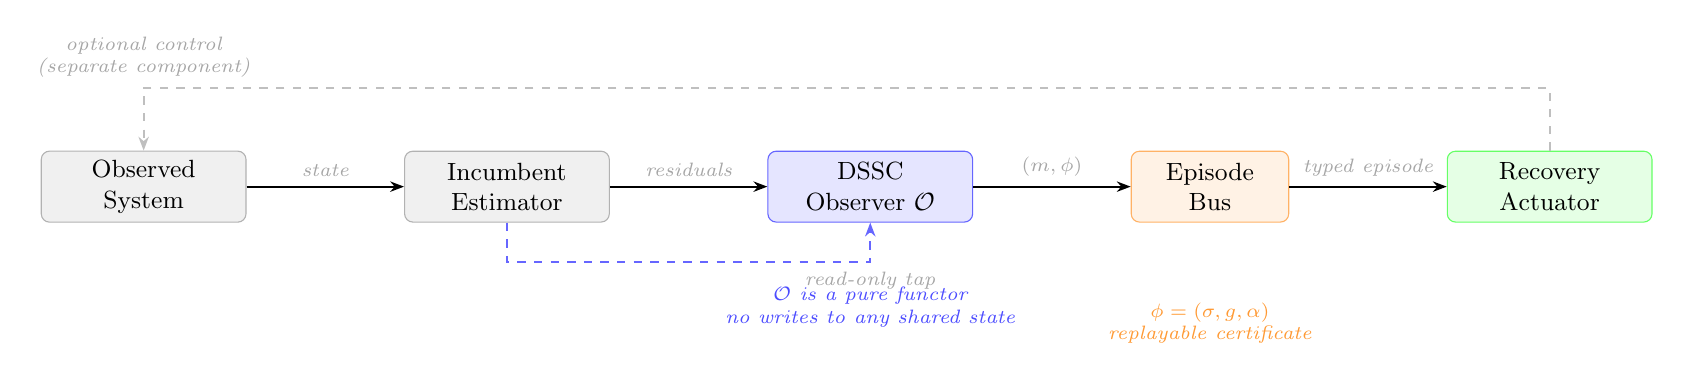
\begin{tikzpicture}[
  node distance=1.4cm and 2.0cm,
  box/.style={draw, rectangle, rounded corners=3pt, minimum width=2.6cm,
              minimum height=0.9cm, align=center, font=\small},
  obs/.style={box, fill=blue!10, draw=blue!60},
  sys/.style={box, fill=gray!12, draw=gray!60},
  act/.style={box, fill=green!10, draw=green!60},
  chan/.style={box, fill=orange!10, draw=orange!60, minimum width=2.0cm},
  arr/.style={-{Stealth[length=5pt]}, thick},
  readonly/.style={-{Stealth[length=5pt]}, thick, dashed, blue!60},
  label/.style={font=\scriptsize\itshape, text=gray!70}
]

% Nodes
\node[sys] (plant) {Observed\\System};
\node[sys, right=of plant] (estimator) {Incumbent\\Estimator};
\node[obs, right=of estimator] (dssc) {DSSC\\Observer~$\Obs$};
\node[chan, right=of dssc] (bus) {Episode\\Bus};
\node[act, right=of bus] (actuator) {Recovery\\Actuator};

% Residual stream
\draw[arr] (plant) -- (estimator) node[midway, above, label] {state};
\draw[arr] (estimator) -- (dssc) node[midway, above, label] {residuals};

% Read-only tap annotation
\draw[readonly] (estimator.south) -- ++(0,-0.5) -| (dssc.south)
  node[midway, below, label] {read-only tap};

% Episode output
\draw[arr] (dssc) -- (bus) node[midway, above, label] {$(m, \phi)$};
\draw[arr] (bus) -- (actuator) node[midway, above, label] {typed episode};

% Optional feedback (dashed, labelled as separate)
\draw[arr, dashed, gray!50] (actuator.north) -- ++(0,0.8) -| (plant.north)
  node[midway, above, label, align=center] {optional control\\(separate component)};

% Non-interference annotation
\node[label, below=0.7cm of dssc, text=blue!70, align=center]
  {$\Obs$ is a pure functor\\no writes to any shared state};

% Provenance chain label
\node[label, below=0.9cm of bus, align=center, text=orange!80]
  {$\phi = (\sigma, g, \alpha)$\\replayable certificate};

\end{tikzpicture}
\caption{DSSC integration architecture. The observer $\Obs$ reads residual streams via a
read-only tap with no feedback path to the observed system (Non-Interference,
Corollary~\ref{cor:noninterference}). A downstream recovery actuator reads typed episodes
$(m, \phi)$ from the episode bus; it is architecturally independent of $\Obs$. Removing
either component leaves the remaining components and the observed system behaviorally
unchanged. The provenance tag $\phi$ in each episode constitutes a DO-178C-eligible audit
certificate (Theorem~\ref{thm:audit}).}
\label{fig:architecture}
\end{figure}

\subsection{The Observer-Only Overlay: Zero-Integration-Risk}

Three additional properties, collectively constituting an \emph{observer-only overlay}
posture, follow directly from the formal results. The critical distinction from every other
diagnostic or monitoring approach is this: \textbf{the DSSC does not ask permission from
the control system, does not modify the control system, and cannot corrupt the control
system.} It is not a co-processor; it is a read-only intelligence layer that sits entirely
outside the safety-critical execution boundary.

\begin{center}
\begin{tcolorbox}[colback=gray!6, colframe=gray!55, boxrule=0.6pt, arc=3pt,
  left=7pt, right=7pt, top=6pt, bottom=6pt,
  title={\textbf{Observer-Only Overlay: Zero-Integration-Risk Properties}},
  fonttitle=\small\bfseries, coltitle=black]
\textbf{R1. Mathematically reversible.}
The observer is a pure functor (Theorem~\ref{thm:functor}, property~4).
Remove it at any time; the controlled system is \emph{mathematically} unchanged --- not
``probably unchanged'' or ``unchanged by policy,'' but provably unchanged by the
functor purity theorem. No rollback procedure is needed because no state was ever modified.
\\[0.3em]
\textbf{R2. No controller access, no architecture review.}
The DSSC reads residual streams already produced by incumbent estimators via a read-only
tap. It does not write to any control register, parameter store, actuator command, or
feedback path. This constraint is enforced structurally by the purity of $\Obs$
(Theorem~\ref{thm:functor}), not by policy or code review. An engineer does not need
to trust that the implementation is non-interfering; the type system proves it.
\\[0.3em]
\textbf{R3. Day-one value with zero configuration.}
With an empty heuristics bank ($h = \emptyset$), the system immediately emits fully
characterized structural episodes (Proposition~\ref{prop:empty_bank}). No training
data, no labeled fault library, no integration testing of the monitoring layer.
Value --- in the form of a deterministic structural log --- begins at the first
residual observation.
\\[0.3em]
\textbf{The licensing ask in one sentence:}
\textit{Add a read-only intelligence layer to your existing residual streams. No
controller access. No architecture change. No rollback risk. Day-one useful.
Removable at any time with zero system impact. Every output is a mathematical proof.}
\end{tcolorbox}
\end{center}

\subsection{Graceful Degradation Posture}

Neural network and ML-based monitoring systems degrade unpredictably under distribution shift:
outputs become uncalibrated, confidence estimates are meaningless, and no certificate of why an
output was produced exists. The DSSC's degradation posture is categorically different:
under heavy-tailed or impulsive noise, the system generates more $\mathtt{Unknown}$ episodes
(Lemma~\ref{lem:graceful_degradation}), each with a complete structural descriptor and a valid
provenance certificate. This is not a limitation to be managed; it is a designed epistemic
honesty property. The operator always knows \emph{exactly} what the system knows and does not
know.

% ============================================================
%  SECTION 11: LIMITATIONS
% ============================================================
\section{Limitations}
\label{sec:limitations}

The DSSC makes no claims beyond the following explicitly stated scope:
\begin{enumerate}[nosep]
  \item \textbf{Discrete-time only.} The calculus assumes $k \in \N$ and does not cover
    continuous-time trajectories.
  \item \textbf{Finite-dimensional residuals.} $V \cong \R^n$ for fixed finite $n$. Infinite-
    dimensional (e.g., functional) residuals are outside scope.
  \item \textbf{Bounded noise (primary regime).} The fragmentation bound (Theorem~\ref{thm:fragmentation})
    requires $\epsilon < \rho_{\min}/2$. Under heavy-tailed noise, Lemma~\ref{lem:graceful_degradation}
    establishes linear degradation in expected fragmentation count, but the strict bound no longer
    holds. The system remains operational and produces valid certificates; it does not crash.
  \item \textbf{$\delta$-band calibration dependency.} The boundary-layer sensitivity parameter
    $\delta$ (Definition~\ref{def:delta_band}) must be set relative to measurement resolution
    at deployment. The formal guarantees hold for any fixed $\delta \in (0, \rho_{\min}/4]$;
    selecting $\delta$ is a calibration task, not a theoretical task.
  \item \textbf{Finite envelope family.} The grammar FSM is finite. Infinite or continuously
    parameterized envelope families require separate treatment.
  \item \textbf{No completeness for arbitrary dynamical systems.} Bounded completeness
    (Theorem~\ref{thm:completeness}) applies only to structurally detectable excursions (those
    that exit the admissibility envelope). Excursions that remain inside the envelope are
    outside the calculus's scope.
  \item \textbf{No domain-specific empirical claims.} All instantiation-specific empirical
    claims appear in domain-specific papers (e.g.,~\cite{dsfb_semi,dsfb_battery}); this paper
    is purely theoretical.
\end{enumerate}

% ============================================================
%  SECTION 12: CONCLUSION
% ============================================================
\section{Conclusion}
\label{sec:conclusion}

We have introduced the DSFB Structural Semiotics Calculus (DSSC), a typed algebraic framework
that unifies the DSFB estimation layer and the ADD modeling layer into a single coherent formal
system, and formalizes \emph{endoduction} as a fourth inference mode alongside the classical
Peircean triad. The seven core theoretical contributions are: a typed syntax for all DSFB
objects; a formal monoidal product on the episode category; a complete deterministic operational
semantics; a category-theoretic observer functor establishing non-interference by construction;
the soundness and bounded completeness proofs for endoduction; the ADD--DSSC integration
theorems; and the graceful-degradation lemma establishing honest operational bounds under
heavy-tailed noise.

Sixteen meta-properties have been proven and collected in Table~\ref{tab:properties}, organized
under six safety-case property codes (SC-1 through SC-6) for direct alignment with DO-178C,
MIL-STD-882E, and IEC~61508 deployment arguments. Every prior DSFB and ADD paper is now a
specialization of this calculus. Future domain papers cite this work for all foundational
definitions and proofs, and describe only the domain-specific instantiation.

Three deployment properties require no additional theoretical work and follow directly as
corollaries of the formal results. (R1)~\textbf{No cold-start problem}: deploying with an
empty heuristics bank immediately produces fully characterized structural episodes; Phase~I
delivers a Deterministic Structural Logger from day one. (R2)~\textbf{Forensic AI}: every
episode carries a provenance tag $\tau_\phi$ that constitutes a replayable mathematical
proof of the diagnostic conclusion, mapping directly to DO-178C, MIL-STD-882E, and
IEC~61508-3 audit requirements. (R3)~\textbf{Observer-only overlay}: read-only by
construction, not by convention; reversible at any time with zero system impact; no
controller access; no architecture review. These are not marketing positions; they are
corollaries of the observer functor (Theorem~\ref{thm:functor}) and totality
(Theorem~\ref{thm:det_total}).

Theoretical directions not pursued here include: higher-order grammars; coalgebraic duals
of the observer functor; continuous-time extensions via differential grammars; and
connections to linear temporal logic for certification-standard property verification.
Each represents a well-posed open problem within the DSSC framework, not a speculative
extension of it.

\vspace{1em}
\textbf{Acknowledgments.} The author acknowledges no external funding. Invariant Forge LLC
is a self-funded independent research entity.

% ============================================================
%  REFERENCES
% ============================================================
\begin{thebibliography}{99}

\bibitem{dsfb_core}
R. de Beer, ``Drift--Slew Fusion Bootstrap: A Deterministic Residual-Based State Correction Framework,''
\textit{Invariant Forge LLC Technical Report}, DOI: 10.5281/zenodo.18706455, 2026.

\bibitem{dsfb_semiotics}
R. de Beer, ``DSFB Structural Semiotics Engine for General Systems: A Deterministic Endoduction Framework for Residual-Based Meaning Extraction,''
\textit{Invariant Forge LLC}, DOI: 10.5281/zenodo.19176473, March 2026.

\bibitem{dsfb_semi}
R. de Beer, ``DSFB Structural Semiotics Engine for Semiconductor Process Control,''
\textit{Invariant Forge LLC}, DOI: 10.5281/zenodo.19413110, March 2026.

\bibitem{dsfb_battery}
R. de Beer, ``DSFB for Battery Health Monitoring,''
\textit{Invariant Forge LLC}, DOI: (deposited), March 2026.

\bibitem{dsfb_nav}
R. de Beer, ``DSFB for Navigation During Plasma Blackout in Hypersonic Re-Entry Vehicles,''
\textit{Invariant Forge LLC}, DOI: (deposited), 2026.

\bibitem{dsfb_survey}
R. de Beer, ``DSFB Structural Semiotics Engine: A Survey of Applications Across Safety-Critical Domains,''
\textit{Invariant Forge LLC}, DOI: 10.5281/zenodo.19204366, March 2026.

\bibitem{add}
R. de Beer, ``Algebraic Deterministic Dynamics (ADD): A Non-Stochastic Structural Extension of DSFB,''
\textit{Invariant Forge LLC}, DOI: 10.5281/zenodo.18830567, March 2026.

\bibitem{dscd}
R. de Beer, ``Deterministic Structural Causal Dynamics (DSCD): Trust-Gated Emergence of Certifiable Causal Graphs for Safety-Critical Aerospace Autonomy,''
\textit{Invariant Forge LLC}, DOI: 10.5281/zenodo.18867217, March 2026.

\bibitem{peirce}
C.~S. Peirce, \textit{Collected Papers of Charles Sanders Peirce}, vols.~I--VIII,
Harvard University Press, Cambridge, MA, 1931--1958.

\bibitem{abduction_ml}
J. Josephson and S. Josephson, \textit{Abductive Inference: Computation, Philosophy, Technology},
Cambridge University Press, 1996.

\bibitem{pac_learning}
M. Kearns and U. Vazirani, \textit{An Introduction to Computational Learning Theory},
MIT Press, Cambridge, MA, 1994.

\bibitem{symbolic_dynamics}
B. Kitchens, \textit{Symbolic Dynamics: One-Sided, Two-Sided and Countable State Markov Shifts},
Springer, 1998.

\bibitem{mbd}
J. de Kleer and B. Williams, ``Diagnosing Multiple Faults,''
\textit{Artificial Intelligence}, 32(1):97--130, 1987.

\bibitem{plotkin_sos}
G. Plotkin, ``A Structural Approach to Operational Semantics,''
\textit{Journal of Logic and Algebraic Programming}, 60--61:17--139, 2004.

\bibitem{pierce_types}
B. Pierce, \textit{Types and Programming Languages}, MIT Press, Cambridge, MA, 2002.

\bibitem{mac_lane}
S. Mac~Lane, \textit{Categories for the Working Mathematician}, 2nd ed., Springer, 1998.

\bibitem{bateson}
G. Bateson, \textit{Steps to an Ecology of Mind}, University of Chicago Press, 1972.

\bibitem{wittgenstein}
L. Wittgenstein, \textit{Philosophical Investigations}, Blackwell, Oxford, 1953.

\bibitem{do178c}
RTCA/DO-178C, \textit{Software Considerations in Airborne Systems and Equipment Certification},
RTCA Inc., Washington, DC, 2011.

\bibitem{milstd882}
MIL-STD-882E, \textit{System Safety}, Department of Defense Standard Practice, 2012.

\bibitem{iec61508}
IEC~61508-3:2010, \textit{Functional Safety of Electrical/Electronic/Programmable Electronic
Safety-Related Systems --- Part~3: Software Requirements}, International Electrotechnical
Commission, Geneva, 2010.

\end{thebibliography}

% ============================================================
%  APPENDICES
% ============================================================
\appendix

\section{Full Proof Sketches}
\label{app:proofs}

\subsection*{Theorem~\ref{thm:det_total}: Determinism and Totality}
The reduction relation is defined by seven SOS rules (Sign-Eval, Env-Eval, Grammar-Adm,
Grammar-Bdy, Grammar-Vio, Enduce, and two composition rules). Each rule fires on a distinct
syntactic form of the head of $P$. The three grammar rules are mutually exclusive by the
partition $\{\interior(E), \partial E, E^c\}$ of $V$ with respect to $E_{\rho(k)}$, which is a
proper partition (boundary has measure zero in $\R^n$; in practice boundary-state is
defined by a $\delta$-band). Enduce is defined on all $(r, \sigma, g, h)$ by the convention
that unmatched patterns return $(\mathtt{Unknown}, \phi)$. Hence the relation is a partial
function (determinism) and is defined on all well-typed configurations (totality). Each
reduction step strictly decreases $|P|$; hence the relation is terminating.

\subsection*{Theorem~\ref{thm:functor}: Observer Functor}
$\Obs$ is well-defined by Theorem~\ref{thm:det_total}. Stationarity: grammar rules depend on
$r(k) \in E_{\rho(k)}$, not on the absolute time $k$; hence shifting the time axis does not
change the grammar sequence. Compositionality: the monoidal product $\otimes$ on $\Ep$ is
defined as episode-sequence concatenation; $\Obs(r_1 \cdot r_2)$ produces the episode sequence
for the concatenated trajectory, which equals the concatenation of episode sequences by the
Markovian grammar property. Purity: by inspection, all SOS rules read from configuration
$\xi$ and produce a new configuration $\xi'$ without any global side-effects; there is no
shared mutable state.

\subsection*{Theorem~\ref{thm:soundness}: Soundness of Endoduction}
By induction on the derivation tree $\phi$. Base case: the $(\mathtt{Unknown}, \phi)$ episode
is trivially sound because it makes no structural claim beyond the structural descriptor.
Inductive case: each motif $m \in M$ is associated in $h$ with a pattern set
$h(m) \subseteq \Sigma^*$; matching fires only when $\sigma[k:k+\ell] \in h(m)$ for some
$\ell$, which is an observed structural fact. The derivation tree $\phi$ records this match,
making the output derivable from the observed trajectory by construction.

\subsection*{Theorem~\ref{thm:completeness}: Bounded Completeness}
By Theorem~\ref{thm:law1}, any trajectory with sustained outward drift exits
$\interior(E_{\rho(k)})$ in time $k^* \leq \lceil \rho_{\max}/d \rceil$. At time $k^*$,
the grammar state is $\mathtt{Bdy}$ or $\mathtt{Vio}$. The Enduce rule fires on any grammar
state, so $\Endo$ executes at $k^*$. By the convention in Definition~\ref{def:endoduction},
$\Endo$ returns either a named motif (if a match exists in $h$) or $(\mathtt{Unknown}, \phi)$
with the full structural descriptor. In both cases, the excursion is characterized. Bounded
completeness does not claim that all excursions are \emph{named} (that depends on $h$); it
claims they are all \emph{characterized}.

\subsection*{Theorem~\ref{thm:fragmentation}: Bounded Fragmentation}
For trajectory $r$, the grammar state is $\mathtt{Bdy}$ when
$r(k) \in E_{\rho(k)} \setminus \interior(E_{\rho(k)})$, i.e., within the boundary layer.
With a $\delta$-band boundary definition, the boundary layer has width $\delta$. The proportion
of time steps at which $r(k)$ lies within $\delta$ of the boundary is bounded by
$2\delta / \rho_{\min}$ under the uniform inner-ball condition. When $r$ and $\tilde{r}$ differ
by at most $\epsilon$, grammar disagreements can only occur when one trajectory is within
$\epsilon$ of the boundary; hence the relative frequency of disagreement is at most
$2\epsilon / \rho_{\min}$, giving the stated bound.

\section{Complete Operator Reference and Transition Tables}
\label{app:operator_ref}

\subsection*{Grammar Transition Table}

\begin{center}
\begin{tabular}{llll}
\toprule
\textbf{Current state} & \textbf{Condition} & \textbf{Next state} & \textbf{Rule} \\
\midrule
$\mathtt{Adm}$ & $r(k) \in \interior(E_{\rho(k)})$ & $\mathtt{Adm}$ & Grammar-Adm \\
$\mathtt{Adm}$ & $r(k) \in \partial E_{\rho(k)}$ & $\mathtt{Bdy}$ & Grammar-Bdy \\
$\mathtt{Adm}$ & $r(k) \notin E_{\rho(k)}$ & $\mathtt{Vio}$ & Grammar-Vio \\
$\mathtt{Bdy}$ & $r(k) \in \interior(E_{\rho(k)})$ & $\mathtt{Adm}$ & Grammar-Adm \\
$\mathtt{Bdy}$ & $r(k) \in \partial E_{\rho(k)}$ & $\mathtt{Bdy}$ & Grammar-Bdy \\
$\mathtt{Bdy}$ & $r(k) \notin E_{\rho(k)}$ & $\mathtt{Vio}$ & Grammar-Vio \\
$\mathtt{Vio}$ & $r(k) \in \interior(E_{\rho(k)})$ & $\mathtt{Adm}$ & Grammar-Adm \\
$\mathtt{Vio}$ & $r(k) \in \partial E_{\rho(k)}$ & $\mathtt{Bdy}$ & Grammar-Bdy \\
$\mathtt{Vio}$ & $r(k) \notin E_{\rho(k)}$ & $\mathtt{Vio}$ & Grammar-Vio \\
\bottomrule
\end{tabular}
\end{center}

\subsection*{Operator Type Signatures}

\begin{center}
\begin{tabular}{ll}
\toprule
\textbf{Operator} & \textbf{Type} \\
\midrule
$\mathtt{sign}$ & $\mathcal{T} \times \N \to \Sigma$ \\
$\mathtt{env}$ & $\Lambda \times \N \to \tau_E$ \\
$\mathtt{inside}$ & $\mathcal{T} \times \N \times \Lambda \to \B$ \\
$\mathtt{transit}$ & $G \times \Sigma \times \N \to G$ \\
$\mathtt{match}$ & $\Sigma^* \times G^* \times \tau_h \to \tau_m \times \tau_\phi$ \\
$\Endo$ & $\mathcal{T} \times \Sigma^* \times G^* \times \tau_h \rightharpoonup \tau_m \times \tau_\phi$ \\
$\mathtt{augment}$ & $\tau_h \times \tau_m \times \mathcal{P}(\Sigma^*) \to \tau_h$ \\
$\mathtt{fuse}$ & $\tau_h \times \tau_h \to \tau_h$ \\
$G_1 \bowtie G_2$ & $\tau_g \times \tau_g$ DFSM product \\
\bottomrule
\end{tabular}
\end{center}

\section{Illustrative Synthetic Derivations}
\label{app:derivations}

This appendix provides three abstract derivation examples demonstrating the DSSC operational
semantics on synthetic trajectories. All trajectories are constructed to be domain-neutral; no
physical system is assumed.

\subsection*{Example 1: Sustained Drift to Boundary}

Let $V = \R$, $E = [-1, 1]$, $r(k) = 0.05k$ for $k = 0, \ldots, 25$.
\begin{itemize}[nosep]
  \item $k = 0$--$18$: $r(k) \in (-1, 1)$ $\implies$ $g(k) = \mathtt{Adm}$; sign $(0.05k, 0.05, 0)$.
  \item $k = 19$: $r(19) = 0.95 \in \partial[-1,1]$ (within $\delta = 0.05$ of boundary)
    $\implies$ $g(19) = \mathtt{Bdy}$.
  \item $k = 20$: $r(20) = 1.00 \in \partial[-1,1]$ $\implies$ $g(20) = \mathtt{Bdy}$.
  \item $k = 21$: $r(21) = 1.05 \notin [-1,1]$ $\implies$ $g(21) = \mathtt{Vio}$.
\end{itemize}
$\Endo$ fires at $k = 21$. Matching against $h$: pattern \texttt{DriftRamp} matches
$(\sigma(0{:}21), g(0{:}21))$. Output: $(\texttt{DriftRamp}, \phi_{21})$.

\subsection*{Example 2: Unknown Structural Event}

Same setup, but with $r(k) = r(k-1) + w(k)$ where $w(k) \in [-0.5, 0.5]$ is non-monotone.
The grammar sequence is $\mathtt{Adm} \to \mathtt{Bdy} \to \mathtt{Adm} \to \mathtt{Bdy} \to
\mathtt{Vio}$ with no persistent pattern. No motif in $h$ matches the fragmented grammar path.
$\Endo$ returns $(\mathtt{Unknown}, \phi)$ where $\phi = (\sigma, g, \alpha)$ is the complete
structural descriptor. The operator is informed: this excursion is structurally characterized
but not yet named.

\subsection*{Example 3: Cross-Stream Fusion}

Let $r^{(1)}(k) = 0.03k$, $r^{(2)}(k) = -0.04k + 0.01k^2$. Individually:
$r^{(1)}$ produces a \texttt{DriftRamp} at $k = 34$; $r^{(2)}$ produces
$\mathtt{Vio}$ at $k = 15$ with a quadratic acceleration signature. The fused observer
$\Obs^{(1,2)}$ fires $\Endo$ on the joint sign sequence and returns a fused episode:
$(\texttt{CrossChannelDivergence}, \phi^{(1,2)})$, a motif not present in either individual
bank but present in the cross-stream bank after augmentation by operational experience.

\subsection*{Example 4: Observer-Driven State Correction (ADD--DSSC Coupling)}

This example demonstrates that while the DSSC observer is non-interfering with respect to
the \emph{observed system}, its typed episode output is high-fidelity enough to drive a
\emph{separate, independent recovery actuator}. The observer and the actuator are distinct
components; the observer writes to no shared state.

\textbf{Setup.} Let $V = \R^2$, $E = B(0, 1)$ (unit ball). A nominal trajectory $r_{\text{nom}}$
satisfies $\norm{r_{\text{nom}}(k)} < 0.8$ for all $k$. A perturbed trajectory
$r(k) = r_{\text{nom}}(k) + d(k)$ where $d(k) = (0.06k, 0)^T$ (sustained drift in the first
component).

\textbf{DSSC observation step.} At each $k$, the observer computes $\sigma(k)$, evaluates
$g(k)$ via the grammar FSM, and emits episodes. At $k^* = 13$:
\begin{align*}
  r(13) &= (\,r_{\text{nom},1}(13) + 0.78,\; r_{\text{nom},2}(13)\,), \quad \norm{r(13)} \approx 0.97 \in \partial_\delta E.
\end{align*}
Grammar state: $\mathtt{Bdy}$. At $k^* = 16$: $\norm{r(16)} \approx 1.06 \notin E$.
Grammar state: $\mathtt{Vio}$. $\Endo$ fires and returns:
\[
  \bigl(\texttt{SustainedDrift\_X},\; \phi_{16}\bigr), \quad
  \phi_{16} = \bigl(\sigma(0{:}16),\; g(0{:}16),\; \alpha_{\text{ADD}}(r)\bigr).
\]

\textbf{Recovery actuator (separate component).} The actuator subscribes to the observer's
episode output channel. Upon receiving
$(\texttt{SustainedDrift\_X}, \phi_{16})$, it reads the provenance tag $\phi_{16}$,
extracts the drift direction from $\sigma$, and issues a correction command
$u_{\text{corr}} = -0.06 \hat{e}_1$ (a counter-drift of equal magnitude). The actuator's
decision logic is:
\begin{equation}
  u_{\text{corr}}(k) \;=\; f\bigl(\Endo(r, \sigma, g, h)\bigr), \quad
  f : \tau_m \times \tau_\phi \to U,
\end{equation}
where $U$ is the actuator's command space. The function $f$ reads the episode type and
provenance; it does not read from $r$ directly.

\textbf{Non-interference verification.} The observer's state $(r, \sigma, g, h)$ is not
modified at any step (purity, Theorem~\ref{thm:functor} property~4). The correction command
flows through a separate channel: observer $\to$ episode bus $\to$ actuator $\to$ plant. If
the actuator is disconnected, the observer continues to emit episodes identically. If the
observer is disconnected, the actuator receives no episodes and issues no commands; the plant
evolves as if neither component were present. The three subsystems are architecturally
independent, sharing only a typed message channel.

\textbf{Provenance chain.} The full derivation chain from disturbance onset to correction
command is:
\[
  d(k) \xrightarrow{\text{trajectory}} r(k)
  \xrightarrow{\Obs} (m, \phi_{16})
  \xrightarrow{f} u_{\text{corr}}
  \xrightarrow{\text{plant}} r_{\text{corrected}}.
\]
Every link in this chain is deterministic and auditable. An engineer can replay the entire
chain from $\phi_{16}$ alone and reconstruct the exact correction issued and why.

\textbf{Implication for certification.} In DO-178C DAL-A software, every output with safety
consequence requires an auditable trace to its inputs~\cite{do178c}. The provenance tag
$\phi_{16}$ constitutes that trace for the recovery command $u_{\text{corr}}$: it is a
complete, replayable derivation certificate requiring no additional logging infrastructure.

\end{document}
